\begin{figure}[t]
	\centering
	\addtolength{\tabcolsep}{-3pt}
	\begin{tabular}{c}
		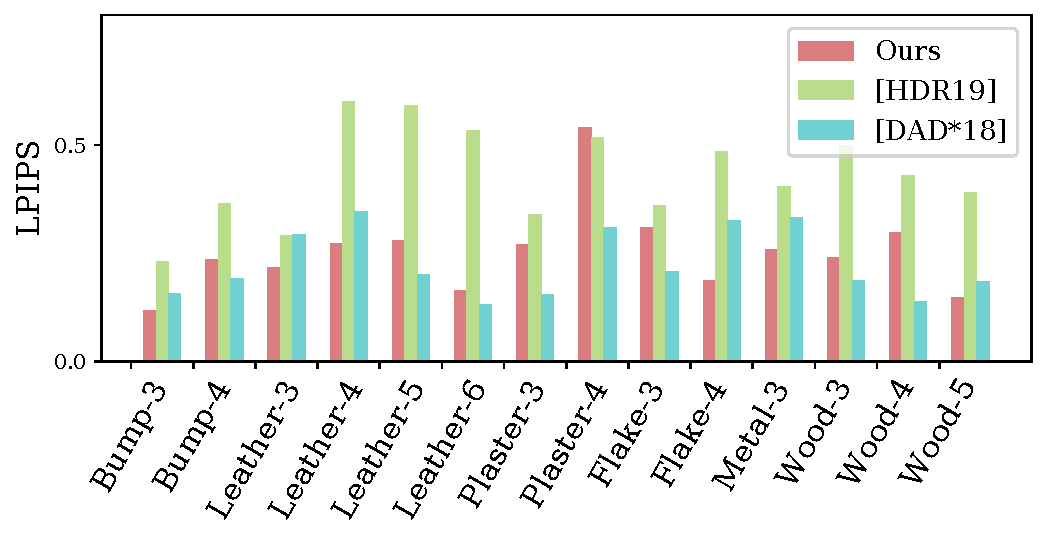
\includegraphics[width=0.9\columnwidth]{img/LPIPS.pdf}
	\end{tabular}
	\captionsetup{labelfont=bf,textfont=it}
	\caption{\label{fig:Comp}
		\revision{
			\textbf{Quantitative evaluation.} The LPIPS of our results are consistently better than \cite{Hu2019}. Some LPIPS values from \cite{Deschaintre2018} are better than ours, since (as per-pixel methods) they can better match the noise patterns in the textures.
		}
	}
\end{figure}